\chapter{Efficient Multi-version Execution}

The key component of multi-version execution system is a runtime monitor that
enables the execution of multiple versions in parallel. Unfortunately, existing
monitors impose either a large performance overhead and/or rely on intrusive
kernel-level changes that increase the size of the trusted computing base.
Moreover, none of the existing solutions scales well with the number of
versions, since the runtime monitor acts as a performance bottleneck.

While synchronization can be performed at different levels, the most common
approach is to do it at the level of system calls, for several different
reasons:  first, many patches do not change the the sequence of system calls,
\ie the program's \textit{external behavior} (\S\ref{sec:behavior-evolution}).
%Second, system calls are the main way in which the application communicates
%with the outside environment, and therefore the ultimate target of attackers.
Second, as the main communication mechanism between applications and the
environment, system calls must be virtualized in order to enable the multiple
versions to act as one to the outside world.

%With the widespread availability of multi-core processors, running multiple
%diversified variants or several different versions of an application in
%parallel is becoming a viable approach for increasing software security and
%reliability.  The key component of such N-version execution (NVX) systems is a
%runtime monitor that enables the execution of multiple versions in parallel.

%In this chapter, we introduce \nx, a multi-version execition framework that
%combines binary rewriting with a novel event-streaming architecture to
%significantly reduce performance overhead and scale well with the number of
%versions, without relying on intrusive kernel modifications.

%Our evaluation shows that \nx can be used to run multi-version applications
%based on a number of popular C10k network servers with only a modest
%performance overhead.

The main challenge in implementing a multi-version execution monitor at the
system call level is the trade-off between performance, security, flexibility
and ease of debugging.  Many
implementations~\cite{orchestra09,tachyon12}, including
Mx (\S\ref{sec:mx}), use the \stt{ptrace} mechanism offered by most UNIX-based
operating systems.  While easy-to-use and not requiring kernel modifications,
\stt{ptrace} is slow, and these systems see performance degradations of up to
two orders of magnitude. A much faster approach is to implement the monitor in
kernel space~\cite{cox2006}, but this requires kernel patches and/or new kernel
modules, and more importantly leads to an increased trusted computing base, as
the monitor runs in privileged mode.  Furthermore, none of these approaches
scale well with the number of variants (as the monitor is both a communication
and synchronization bottleneck), none are debug-friendly (\stt{ptrace}
disallows the use of \stt{gdb}, while kernel debugging has its well-known set
of limitations) and none of them have been designed to be flexible with respect
to small variations in system call sequences (which can occur for certain
diversification transformations and across program versions).

%In this chapter, we introduce \nx, a multi-version execution framework that
%combines binary rewriting with a novel event-streaming architecture to
%significantly reduce performance overhead and scale well with the number of
%versions, without relying on intrusive kernel modifications.

In this chapter, we introduce \nx,\footnote{\varan's name comes from the
scientific name \emph{Varanus}, commonly known as the \emph{monitor} lizard.
Varan is also a name of the Kaiju monster that first appeared in the 1958 movie
\emph{Varan the Unbelievable}.} a multi-version execution system that
combines binary rewriting with a novel event-streaming architecture to
significantly reduce performance overhead and scale well with the number of
versions, without relying on intrusive kernel modifications. \nx monitor
operates at the system call level, runs in user space (and therefore in
unprivileged mode), introduces a small performance overhead for popular C10k
network servers and negligible for CPU-bound applications, scale well with the
number of versions, and provide a flexible mechanism for handling small
divergences in the system calls sequences issued across versions.

\section{Overview}
\label{sec:overview}

Two key aspects influence the performance and flexibility of an NVX
system: system call interception and version coordination.  We discuss
each in turn below.

\subsection{System call interception}
\label{sec:interception}

%% \begin{enumerate}[(i)]
%% \item wait for the interrupt signaling the entry to a system call;
%% \item examine the registers to determine whether the system
%% call is of interest;
%% \item for any arguments passed by reference, copy the content of
%% the memory for the process address space if necessary;
%% \item if the system call is to be skipped (or performed by the monitor
%% on behalf of the application), replace the original system call with a
%% "null" system call (\ie \lstinline`getpid`);
%% \item restart the execution of the application to execute the system call;
%% \item wait for the interrupt signaling the exit from a system call;
%% \item obtain the process registers to read the system call return value;
%% \item for any output arguments, copy the referenced data from
%% the process address space if needed; and
%% \item continue the execution of the application.
%% \end{enumerate}

The biggest downside of existing system call monitors based on the
\ptrace interface is the high performance
overhead~\cite{orchestra09,tachyon12}.  For each system call
performed by each version, execution must switch to the monitor
process, which has to perform several additional system calls in order
%to be notified about system call entry and exit, 
to copy buffers to and from the version being monitored, nullify the
system call, \etc as shown earlier in
Figure~\ref{fig:lockstep-execution}.

For CPU-intensive applications which perform few system calls, this
overhead will be amortised, translating into a modest overall
slowdown.  However, for heavily I/O-bound applications, the slowdown
can be up to two orders of magnitude, which is unacceptable for many
real-world deployments.
%
Consequently, in order to implement a system call monitor with
acceptable overhead even for heavily I/O-bound applications, we need
to eliminate context switching to the monitor and back during
interception and eliminate the need for additional system calls.  
This is accomplished through a combination of selective binary
rewriting and an interprocess communication mechanism based on a
fast shared memory ring buffer.

%\vspace{0.1in} \noindent \textbf{Selective binary rewriting.}  
Whenever code is loaded into memory, \varan scans each code page to
selectively rewrite all system calls with jump instructions to dedicated
handlers.  Section \ref{sec:rewriting} discusses in detail the main
steps and challenges associated with this binary rewriting approach.

To eliminate the need for additional system calls during interception,
\varan uses a shared ring buffer to communicate between versions.  This
ring buffer is heavily optimised for performance: it is stored in
memory, allows largely lock-free communication, and does not require
the dispatch of events to different queues.  These aspects are
discussed in detail in Section~\ref{sec:streaming}.



\subsection{Event-streaming architecture}
\label{sec:coordination}

In prior NVX systems, versions are typically run in lockstep, with a
centralised monitor coordinating and virtualising their execution.
Essentially, at each system call, the versions pass control to the
monitor, which waits until all versions reach the same system call.
Once this happens, the monitor executes the system call and
communicates the result to each individual version.  If two or more
versions try to break the lockstep by executing different system
calls, the monitor needs to either terminate the entire application or
continue executing a subset of the versions in lockstep.

This approach has two key disadvantages.  First, the centralised
monitor is a bottleneck, which can have a significant impact on
performance.  Note that in addition to the synchronisation overhead,
this centralised monitor makes the NVX application execute at the
speed of the slowest individual version.

Second, this approach is totally inflexible to any divergence in the
sequence of system calls executed across versions.  This is an issue
both when running automatically-diversified variants, where certain
transformations may affect the external behaviour, and when running
existing software revisions, where changes in the sequences of
system calls can occur between revisions. 

\begin{figure}[t]
  \begin{center}
    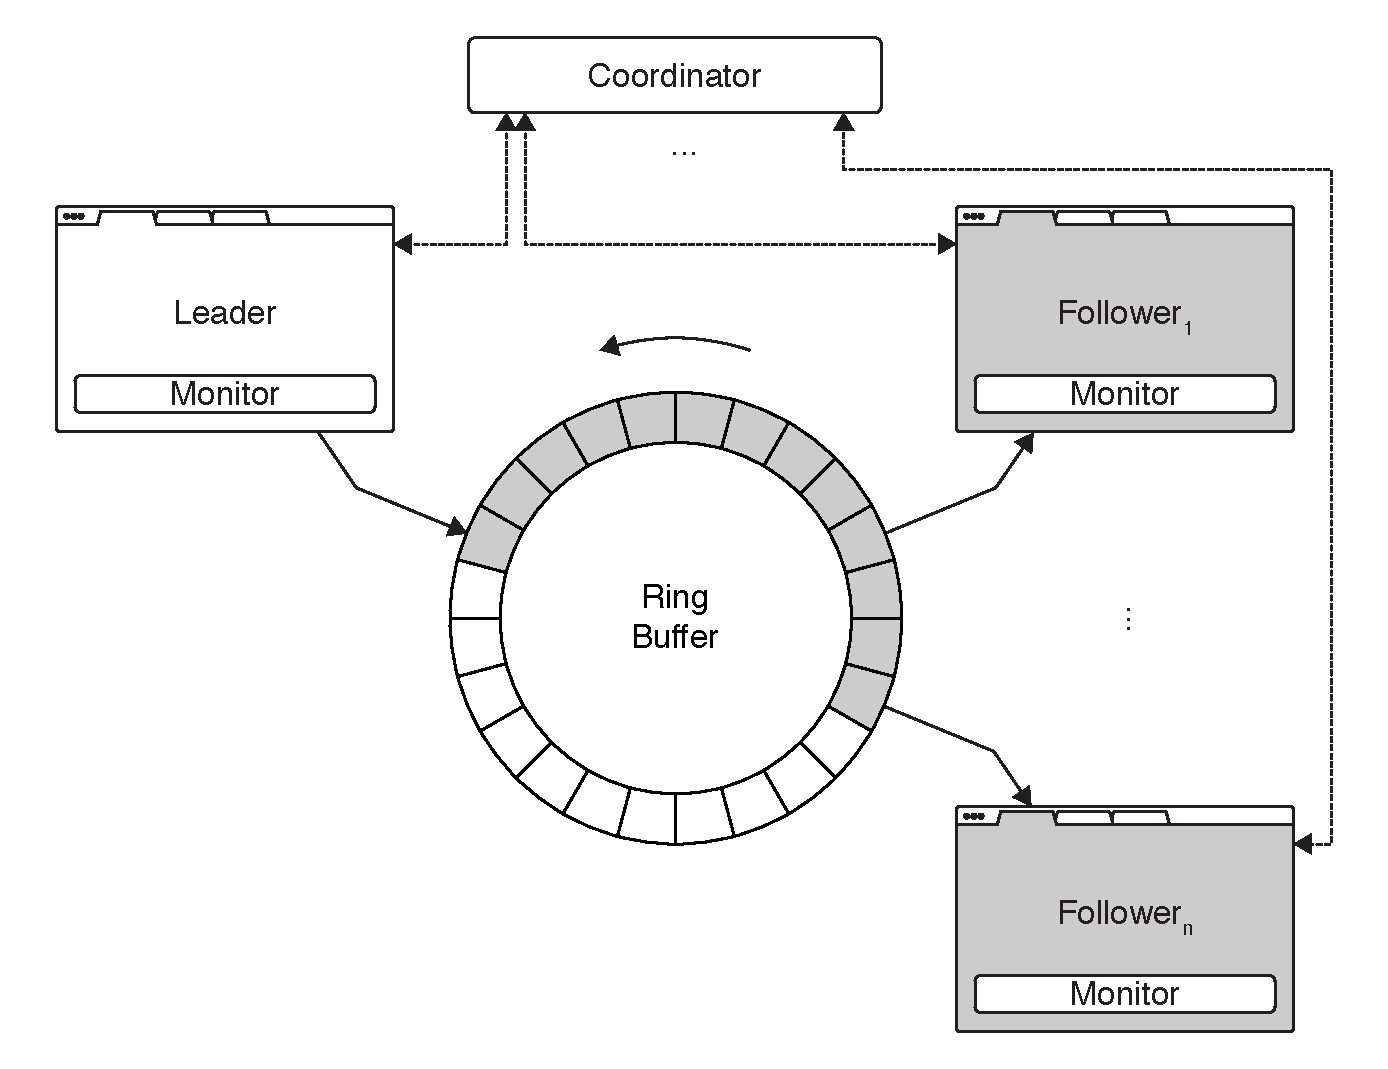
\includegraphics[width=0.6\textwidth]{efficient-execution/figures/architecture}
    \caption{The event-streaming architecture of \varan.}
    \label{fig:architecture}
  \end{center}
\end{figure}

To address these limitations, \varan uses a new approach which we call
\emph{event streaming}.  In this decentralised architecture,
depicted in Figure~\ref{fig:architecture}, one of the
versions is designated as the \textit{leader}, while the others are
\textit{followers}. During execution, the leader records all events into a
shared ring buffer, which are later read by followers to mimic the leader's
external behaviour (\S\ref{sec:streaming}). Events consist primarily
of regular system
call invocations, but also of signals, process forks (\ie \lstinline`clone`
and \lstinline`fork` system calls) and exits (\ie \lstinline`exit` and
\lstinline`exit_group` system calls).

In general, any version can be the leader, although in some situations
some may be a better choice than others, \eg when running multiple
software revisions in parallel, one might prefer to designate the
newest one as leader.  However, the leader can be easily replaced if
necessary, \eg if it crashes (\S\ref{sec:leader-repl}).

The only centralised component in this architecture is the
\textit{coordinator}, whose main job is to prepare the versions for
execution and establish the necessary communication channels.  At a
high level, the coordinator first loads the variants into memory,
injects several special handlers and memory objects into their address
spaces, rewrites any system calls in their code with jumps to the
special handlers and then starts executing the variants
(\S\ref{sec:setup}) in a decentralised manner.

%% recorded by one application version are shortly replayed
%% (\textit{streamed}) to the others, which keeps the log small, as
%% events which have been replayed by all versions can be discarded.
%% Similarly, the NVX context allows for the log to be kept in memory,
%% and for the replay to be done incrementally, with significant
%% performance advantages.  Event streaming is discussed in detail in
%% Section~\ref{sec:streaming}.


%% This is a variant of record-replay~\cite{scribe,jockey,geels06,r2},
%% but the NVX context allows us to overcome two of the main limitations
%% of traditional record-replay techniques, namely (1)~the
%% rapidly-growing log size, especially for system call-intensive
%% applications; and (2)~the long time necessary to replay the execution.
%% Because the multiple versions are executed concurrently, events
%% recorded by one application version are shortly replayed
%% (\textit{streamed}) to the others, which keeps the log small, as
%% events which have been replayed by all versions can be discarded.
%% Similarly, the NVX context allows for the log to be kept in memory,
%% and for the replay to be done incrementally, with significant
%% performance advantages.  Event streaming is discussed in detail in
%% Section~\ref{sec:streaming}.


\subsection{Rewrite rules for system call sequences}
\label{sec:rw}

In addition to eliminating the central monitor bottleneck, our
event-streaming architecture also supports (small) divergences between
the system call sequences of different variants.  For example,
different software revisions can be run inside a classical NVX
system only as long as they all issue the same sequence of system
calls~\cite{mx}.  However, software patches sometimes change the
external behavior of an application.  In particular, many divergences
in system call traces fall into the following two categories:
\begin{inparaenum}[(i)]
\item \emph{addition/removal}, characterising situations when one of
  the versions performs (or conversely does not perform) an additional
  system call, typically as a consequence of an additional check, and
\item \emph{coalescing}, covering the situations when a (repeated)
  sequence of system calls is executed a different number of times in
  each version (\eg one version might execute two \lstinline`write`
  system calls, while another version executes only one
  \lstinline`write` system call to write the same bytes because extra
  buffering is used).

\end{inparaenum}

% \begin{description}
%   \item[Addition/Removal] This class characterises situations when one
%     of the versions performs an additional system call (or conversely
%     does not perform), typically as a consequence of an additional
%     check.
%   \item[Coalescing] This class covers the situations when a (repeated)
%     sequence of system calls is executed a different number of times
%     in each version.  E.g., one version might execute two \lstinline`write`
%     system calls, while another a single equivalent \lstinline`write` to
%     write the same bytes (\eg because extra buffering is used).  
% \end{description}

\varan is the first NVX system that is able to deal with such changes.
When followers process the event sequence streamed by the leader, they
can rewrite it to account for any such differences: \eg they can skip
and merge system calls, or perform some calls themselves.  We provide
a flexible implementation of such rewrite rules using Berkeley Packet
Filters (\S\ref{sec:patternmatching}).


\section{\vx Prototype System}
\label{sec:prototype}

%% \begin{figure}[t]
%%   \begin{center}
%%     \includegraphics[width=\columnwidth]{figures/process-model}
%%     \caption{\vx process model.}
%%     \label{fig:process_model}
%%   \end{center}
%% \end{figure}

\begin{figure*}[t]
  \begin{center}
    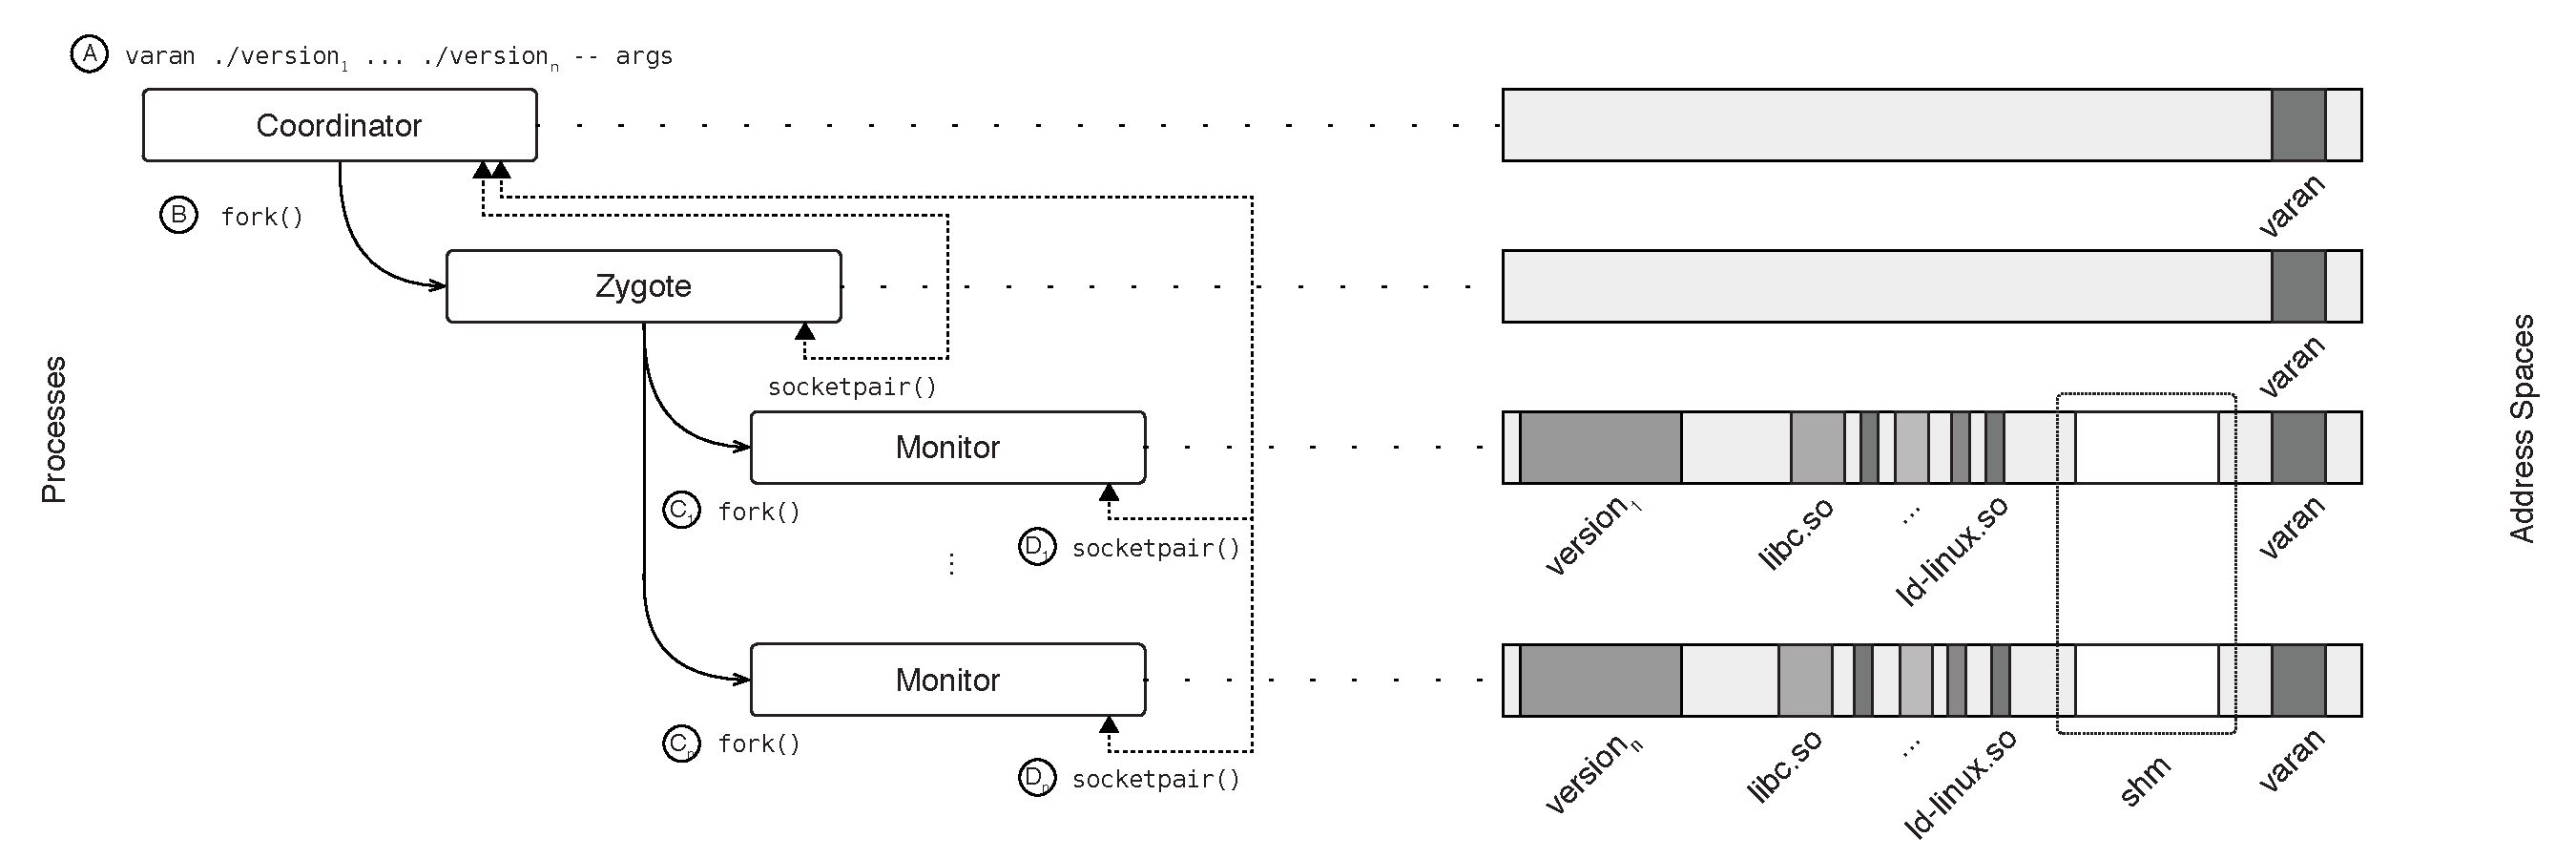
\includegraphics[width=\textwidth]{efficient-execution/figures/address-space}
    \caption{Setup of address spaces and communication channels.}
    \label{fig:setup}
  \end{center}
\end{figure*}


We have implemented our approach in a prototype, to which we will
refer as \vx, targeted at multi-core processors running x86-64 Linux.
\varan works on off-the-shelf binaries (both stripped and unstripped)
and supports single- as well as multi-threaded applications.

When it starts, \vx first sets up the address spaces of all program
versions and establishes the needed communication channels
(\S\ref{sec:setup}).  It then performs selective binary rewriting to
replace all system calls with  jump instructions
(\S\ref{sec:rewriting}).  After these initial stages, the event
streamer component of \vx ensures the coordination of the leader and
its followers (\S\ref{sec:streaming}).


\subsection{Setup of address spaces and communication channels}
\label{sec:setup}

The main steps involved in the setup of version address spaces and the
needed communication channels are shown in Figure~\ref{fig:setup}.  To
run multiple versions in parallel, the user launches \vx providing the
paths to all versions, together with any command line arguments required
to start them (Step \circl{A} in Figure~\ref{fig:setup}). \vx is built
as a statically-linked, position-independent library, to make sure it
does not stand in the way of any segments which have to be loaded by the
application at fixed addresses.

% \begin{lstlisting}[language=bash,numbers=none]
% varan -p /path/to/executable1 
%         -p /path/to/executable2 -- args
% \end{lstlisting}

%The coordinator is linked with the \vx library (\vxlib, stored in
%\stt{libvaran.so}), which will be also injected inside each version.
%\vxlib is built as a statically-linked, position-independent library,
%to make sure it does not stand in the way of any segments which have
%to be loaded by the application at fixed addresses.

The \emph{coordinator} code first creates the shared memory segment
used for communication among versions, and then spawns the
\textit{zygote} process (\circl{B}), which is responsible for starting
the individual versions. The coordinator communicates with the zygote
via a UNIX domain socket. For each version $i$ that needs to be spawned,
the coordinator sends a fork request to the zygote over this socket
pair, which includes the path to that version executable, the command
line arguments, and the end-point of a socket pair which will be used
for the subsequent communication between the coordinator and that
version (\circl{C$_i$}).
%
After receiving this request, the zygote spawns a new process, which
first finalizes the communication with the coordinator
(\circl{D$_i$}).  The coordinator then sends the shared memory
segment descriptor to this process, which maps it inside its address
space.

%% returns a process identifier to the coordinator.  The coordinator then
%% sends the rank and shared memory segment descriptor to the version.

In the final step, the new process starts executing inside the
\emph{monitor} code, which loads the specified ELF executable and sets
up the initial address space as described in the ELF headers. If the
program requires a dynamic linker, \vx loads the linker image specified
in the header as well.
%% Afterwards, \vx attaches the shared memory segment and initializes
%% the system call table based on the rank and arguments provided by
%% the coordinator.
The text segments of both the application and the dynamic linker are
then processed by the binary rewriter (\S\ref{sec:rewriting}). Finally,
\vx jumps to the application entry point as specified in the ELF header,
starting the execution of the application version.

%% \vx is operates at the thin boundary between the operating system and
%% the user-space application---\ie below the C library and the dynamic
%% linker---and lives inside the address space of the host application;
%% however, the application itself is unaware of its existence.

% The rest of this section provides some extra details regarding the
% role and implementation of the coordinator, monitor and zygote.

\boldtext{Coordinator.}  Essentially, to set up the address spaces of
the versions, the coordinator acts as a specialized preloader, inspired
by
\emph{rtldi}.\footnote{\url{http://www.bitwagon.com/rtldi/rtldi.html}}
However, the coordinator does not attempt to replace the existing
dynamic linker, which would be unnecessarily complex and may affect
compatibility with existing applications. Instead, it simply intercepts
system calls performed by the linker to enable the binary rewriter
(discussed in \S\ref{sec:rewriting}) to rewrite the code of
dynamically-linked shared libraries.  One important advantage of our
interception mechanism is that we do not make use of \ptrace to
intercept calls to the dynamic linker---instead, the binary rewriter is
used to rewrite all the system calls done by the linker with jumps into
the coordinator code.  As a result, \vx can be used in combination with
existing \stt{ptrace}-based tools such as \textit{GDB} or
\textit{strace}, which greatly simplifies debugging.

%% This also has an advantage of supporting arbitrary dynamic linkers,
%% not just the one provided by GNU C library, albeit it is going to be
%% the most common target.

%% This architecture has several advantages over other commonly
%% approaches. \vx does not require the use of dynamic linker, as
%% required by \stt{LD\_PRELOAD}. 


\boldtext{Monitor.} To ensure that \vx can be compiled as
statically-linked position-independent code, we must avoid using any
global variables (\ie those in the \stt{.data} section). One of the
consequences is that \vx cannot use any of the existing C libraries such
as \textit{GNU C Library}, as these are not typically built to support
this requirement.  Instead, \vx provides its own implementation of the
necessary C library functions based on the \textit{Bionic C
library}.\footnote{\url{https://android.googlesource.com/platform/bionic.git}}
To support the use of Linux system calls, \vx uses a modified version of
the \stt{linux\_syscall\_support.h}
header.\footnote{\url{https://code.google.com/p/linux-syscall-support/}}

%% \vxlib provides its own entry point (\ie the \stt{\_start} function),
%% which is the starting point for \vx's execution. After start, it first
%% processes the arguments passed on stack by the Linux kernel, including
%% program arguments, environment variables and most importantly the
%% auxiliary data. Then, it loads the specified ELF executable into the
%% address space. Since \vx operates as a pre-loader, it is responsible
%% for setting up the initial address space layout as described by the
%% program header. If the program being executed requires dynamic linker,
%% \vx loads the linker image specified in the program header as
%% well. The text segments of both the application and the dynamic linker
%% are then processed by the binary rewriter (\S\ref{sec:rewriting}).


\boldtext{Zygote.} While it would be technically possible for the coordinator
to create the processes in which versions run, instead of delegating this
functionality onto the zygote, this would bring some complications regarding
the communication channels: for example, the second version spawned would
inherit the communication channel between the first version and the
coordinator, which would be undesirable.  Zygote processes are already used in
popular systems such as \textit{Android} and
\textit{Chrome}~\cite{linuxzygote}---in this paper, we use the term to refer to
the concept rather than a concrete implementation, as \vx provides its own
clean-slate implementation.

After start, \vx sets up the communication subsystem (\ie the shared memory
allocator, the ring buffer) and then forks the Zygote process. The Zygote
closes all open descriptors except for the socket used as a communication
channel with the coordinator and enters the dispatch loop to wait for incoming
requests. On fork request, the Zygote receives command line arguments (\ie
\stt{argv}) and a set of file descriptors which will be available to the new
process; then forks itself and resumes to dispatch loop. The other type of
requests that Zygote supports are querying for process status (\ie equivalent
of \stt{waitpid}) and process termination (\ie \stt{SIGKILL}).

\subsection{Binary Rewriting}
\label{sec:rewriting}

To intercept system calls, \vx uses selective binary rewriting~\cite{bird}.
Unlike traditional dynamic binary rewriting implemented by tools like
DynamoRIO~\cite{dynamorio02} or Pin~\cite{pin05}, where the entire process
image is being rewritten often introducing significant performance overhead,
\vx only replaces certain instructions, in particular the instructions for
performing system calls (\ie \stt{INT 0x80} on x86 and \stt{SYSCALL} on
x86-64).  This approach has been originally implemented in
\emph{BIRD}~\cite{bird} for the Windows/x86 platform and later in
\emph{seccompsandbox}\footnote{\url{https://code.google.com/p/seccompsandbox/}}
for Linux.  Our implementation extends the
\emph{seccompsandbox}\footnote{\url{https://code.google.com/p/seccompsandbox/}}
framework for Linux.

The rewriting itself is done statically when a text segment is mapped into
memory.  (\ie \stt{mmap} system calls with executable flag, typically performed
by the dynamic linker).  \vx iterates through the text segment searching for
system call instructions using a simple x86 disassembler. Every system call
found is rewritten with a jump to an internal system call entry point. This
process is complicated by the fact that while a system call instruction is only
one byte long, a jump instruction requires five bytes. Therefore, in order to
rewrite the system call with a jump, we also need to relocate some of the
instructions surrounding the system call---\ie perform binary detouring via
trampolines~\cite{detours}.  On rare occasions when this is not possible (\eg
because the surrounding instructions are potential branch targets), we replace
the system call with an interrupt (\stt{INT 0x0}).  This interrupt is handled
by \vx through a signal handler installed during initialization, which
redirects the control flow to the system call entry point as for other system
calls.

The system call entry point first saves all registers, and then checks an
internal system call table to see whether there is a handler installed for that
particular system call; if so, it calls that handler (using a user space
calling convention), otherwise it invokes the default handler.  After
processing the system call, the entry point handler restores all registers and
returns to the original caller (using \stt{sigreturn} in the case of system
calls intercepted via an interrupt). The system call entry point also
implements support for restarting system calls, normally handled by the kernel
(\ie signaled by the \stt{-ERESTARTSYS} error code). This is used in certain
scenarios supported by \vx such as transparent failover (\S\ref{sec:failover}).

The internal system call table can be easily changed to accommodate
various application scenarios.  In particular, the only difference
between the leader and the followers is the system call table. For
example, the \stt{write} system call would be redirected in the leader
to a function that performs the call and records its result in the
shared ring buffer, while in the followers it would be redirected to a
function that reads the results from the shared buffer without making
the call.
%% \vx allows both the system call table and the default system call
%% handler to be provided by the embedder of \vx \todo{Where shall we
%%   described the possibility of \vx embedding, \ie building tools on
%%   top of \vx?}. This makes it easy to customize \vx behavior for
%% different use cases (\S\ref{sec:failover}). For our prototype, we have
%% provide three different system call tables (\ie record, replay and
%% passthrough). 
\varan  also provides a Python script which can produce new tables
and their implementations using templates.
%% ; in fact, the passthrough table was implemented using this
%% generator. We have also used the generator throughout the \vx
%% development for testing and debugging purposes.


\subsubsection{Virtual System Calls}
\label{sec:vsyscall}

The \emph{vsyscall} page and the \emph{vDSO} segment are two
mechanisms used to accelerate certain system calls in Linux. Each
process in Linux has two special segments mapped into its address
space, containing virtual system call implementations. These system
calls do not incur the context switch overhead between kernel and
user space associated with "standard" system calls.

The \emph{vsyscall} page was introduced first, but is being deprecated in favor
of the \emph{vDSO} segment.\footnote{We are referring to x86-64 version, on x86
the vDSO segment contains a function used to determine the preferred method of
making a system call} The main reason for this development is that the
\emph{vsyscall} page is mapped to a fixed address, making it susceptible to
return-oriented programming attacks~\cite{ROP:tissec12}. To address this issue,
the vDSO segment is mapped to a random address. Since the segment is
dynamically allocated, it can also support an arbitrary number of virtual
system calls (currently \stt{clock\_gettime}, \stt{getcpu}, \stt{gettimeofday}
and \stt{time}).

Virtual system calls represents one of the major limitations of
\stt{ptrace} based monitors. Since these system calls are entirely
implemented in user space, they cannot be intercepted via \ptrace.
This is an important limitation: as these system calls provide access
to timing information, they are often used as a source of
non-determinism (\eg for random number generators) and their handling
is critical for any NVX system. Despite this, previous systems either
omit discussion on virtual system call handling~\cite{mx,orchestra11}
or explicitly mention their inability to handle them~\cite{tachyon12}.

To our knowledge, \vx is the first NVX system which handles virtual
system calls, using binary rewriting. 
%In \vx, binary rewriting is also used to intercept virtual system
%calls.
Handling calls made via the \textit{vsyscall} page is easier, as
the function symbols are always mapped at the same address.  
We can therefore easily identify calls to these functions while
scanning the text segment and rewrite them to calls into our system
call table.
To handle \textit{vDSO} calls, we first need to
determine the base address of the \textit{vDSO} segment; this address
is passed by the kernel in the ELF auxiliary vector via the
\stt{AT\_SYSINFO\_EHDR}
flag.\footnote{\url{https://www.gnu.org/software/libc/manual/html_node/Auxiliary-Vector.html}}
Second, we need to examine the ELF headers of the \textit{vDSO}
segment to find all symbols.  Since these symbols are allocated at
arbitrary addresses, statically identifying calls to these symbols as
in the \textit{vsyscall} case would be complicated. Instead, we
replace the entry point of each function with a jump to dynamically
generated code which sets up the stack and then issues a call to the
\vx system call entry point as in case of regular system
calls. Furthermore, we provide a trampoline, which allows the
invocation of the original function, by moving the first few
instructions of each function to a new place, followed by a jump to
the original code. This allows \vx to take advantage of the virtual
system call mechanism to further improve performance.

%% Finally, we note that this function interception mechanism is not
%% specific to system calls and can be used to intercept arbitrary
%% functions in the target application if needed, similarly to
%% Detours~\cite{detours}.



\subsection{Event Streaming}
\label{sec:streaming}

As briefly discussed in Section~\ref{sec:overview} and graphically
illustrated in Figure~\ref{fig:architecture}, the leader records all
external events into a shared ring buffer, while the followers replay
them to mimic the leader's behavior.  External events consist
primarily of system call invocations, but also of signals.  The leader
is the only version interacting with the environment, \ie executing
the system calls, with exception of system calls which are local to
the process (\eg \stt{mmap}). % or \stt{sigaction}).

As in any NVX system operating at the level of system calls, \vx has
to be aware of the system call semantics, in order to transfer the
arguments and results of each system call.  \vx currently implements
\syscallsHandlers system call handlers which were specifically selected
to cover the common operations (file and network I/O, event
notification, process management). This has proven enough to
successfully run all applications used in our evaluation.

%, with the remaining system
%calls allowed to be executed directly by each version, which has
%proven enough to successfully run all the servers used in our
%evaluation.

%% All application instances running in parallel under \vx are assigned
%% ranks, similarly to OpenMPI~\cite{OpenMPI}. The instance\footnote{We
%%   refer to the instances rather than a process as application may have
%%   multiple threads/subprocesses} with rank 0 is denoted as
%% \emph{leader} while all other instances are denoted as
%% \emph{followers}. 


%% When followers would execute a system call under normal execution, now
%% they simply return a value from the event stream (\ie the return value
%% of the system call executed by the leader).

% \vx recognizes several different types of events:
% \begin{inparaenum}[(i)]
% \item \emph{syscall} for the system call entry,
% \item \emph{sysret} for the system call exit,
% \item \emph{signal} for an interceptable signal,
% \item \emph{exit} for the process exit.
% \end{inparaenum}
% Furthermore, it is possible to add other types of events if necessary.

%% Each event has a fixed size of 64 bytes where first byte is
%% used as an event type.  The size has been deliberately chosen to be
%% fit into a single cache line on modern x86 CPU (see \S\ref{sec:ipc}
%% for more details).

\subsection{Inter-process Communication}
\label{sec:ipc}

%% \begin{structure}
%% \item Sending events from one process to other without the use of system
%% calls to avoid the additional overhead
%% \item Shared memory queues for process to process communication
%% \item Custom shared memory allocator with reference counting
%% \end{structure}

Since one of our primary goals for \vx was to minimize the performance
overhead, to avoid additional system calls being made during system call
handling (\S\ref{sec:overview}), we have designed an interprocess communication
mechanism which does not use system calls (\eg socket-based communication
primitives).

\subsubsection{Shared ring buffer}
\label{sec:ring}

For fast communication, the leader and its followers share a common
ring buffer of fixed size, which is held entirely in memory.  Our
initial solution used a separate shared queue for each
process~\cite{fastforward,mcringbuffer}, with the
%% Shared memory queues are often used for fast core-to-core
%% communication in high-performance applications.
coordinator acting as an event pump---reading events from the leader's
queue and dispatching them into followers' queues.  This approach
worked well for a low system call rate, but at higher rates the event
pump quickly became a bottleneck.  
% Furthermore, although we used a
% state-of-the-art shared queue implementation~\cite{bqueue}, we still
% experienced a large performance overhead for system call
% interception---over $20\times$ for a worst-case microbenchmark,
% compared to $4\times$ in the final implementation.

As a result, we have instead opted for a design based on Disruptor
pattern~\cite{disruptor} which uses a shared ring buffer allowing concurrent
access by multiple producers and consumers, eliminating the need to dispatch
events among queues, and thus improving both performance and memory
consumption.  Our implementation uses C11 atomics, 
in combination with cache aligning to
achieve maximum performance with minimal use of locking (locks are used only
during memory allocation and deallocation).

The ring buffer is used to stream events between processes. Each event
has a fixed size of 64 bytes; the size has been deliberately chosen to
fit into a single cache line on modern x86 CPUs.  This is sufficient
for sending signals and system calls for which all arguments are
passed by value (on x86-64, a system call can have up to six arguments
of eight bytes, to fit into general purpose registers).  However, for
system call arguments passed by reference, the payload might have
variable size and can be potentially larger than the event itself.  In
this case, we use events to only transfer shared pointers, which
identify memory shared across versions.


\subsubsection{Transferring file descriptors and leader replacement}
\label{sec:leader-repl}

Apart from the ring buffer, each version has a \textit{data channel},
implemented using UNIX domain sockets.
% Together, the ring buffer and data channel form an \emph{event
% stream} which is a primary communication mechanism for exchanging
% events among instances.
The data channel is used to send information which cannot be
transferred via shared memory, in particular open file descriptors.
Whenever the leader obtains new file descriptor (\eg by opening a
file), it sends this descriptor to all followers, effectively
duplicating the descriptor into their processes. This is a crucial
mechanism which enables the leader to be replaced transparently when
it crashes. When the leader crashes, the follower that is elected as
the new leader can simply continue executing using existing
descriptors (\eg responding to requests coming over network) without
any disruption in service.

% Currently, UNIX domain sockets do not support broadcast, so the leader
% communicates with the followers via the coordinator, which then sends
% the descriptor separately to all followers.  However, there are
% proposals to add broadcast support for UNIX domain
% sockets,\footnote{\url{https://lkml.org/lkml/2012/2/20/208}} which would
% simplify the design of our prototype and further improve performance.


\subsubsection{Multi-process and multi-threaded applications}
\label{sec:threading}

Handling threads is crucial in supporting many modern applications. To
alleviate non-determinism issues due to scheduling, \vx enforces
system call ordering across all threads in all variants by using a
single shared ring buffer.  Each event sent through the ring buffer is
annotated with an internal thread ID. When reading events from the buffer, each
thread checks the ID of every new event and blocks if the event ID does not
match its own.  Since our ring buffer implementation (\S\ref{sec:ring}) allows
concurrent writes by multiple producers without the need for expensive
synchronization, the use of a single shared buffer does not hinder the
application performance. 

When a new thread is spawn, a new socket pair is established between the thread
and the coordinator. The leader then continues execution, but the coordinator
waits until all followers spawn a new thread, establishing appropriate socket
pairs for communication, and setting up the thread to read events from the
shared ring buffer.

Our mechanism resembles existing deterministic multi-threading (DMT)
mechanisms~\cite{coredet:asplos10,dthreads:sosp11}. The guarantees
provided by \vx are weaker than those typically provided by these
systems as we do not enforce ordering across atomics-based
synchronization primitives.

The use of a single shared buffer presents a problem when one or more threads
perform a system call which blocks for a long period of time. In such case, the
other threads could run out of space in the ring buffer. Since the ring buffer
uses busy waiting, the following threads would also waste resources. To overcome
this problem, we have introduced a concept of \emph{waitlock}. Whenever the
following thread makes a blocking system calls, it acquires the waitlock. Such
thread is no longer holding a position in the ring buffer and it blocks until it
receives a notification from the leading thread when the waiting thread wakes up
and continues execution. The waitlocks are internally implemented using a
combination of C11 atomics and futexes~\cite{futex} for efficiency.

% However, this weaker form of determinism
% does not typically pose a problem for real-world applications as long
% as they are properly synchronized.  Note that data races resulting
% from missing or incorrect synchronization can cause followers to issue
% a different sequence of system calls from the leader.  If this
% happens, we could either try to apply one of the rewriting rules
% (\S\ref{sec:patternmatching}), or terminate the follower.
%
However, we have not detected any system call divergences caused by
related data races in our benchmarks, which include multi-threaded
applications (\eg \redis), similar to the experience reported for
prior NVX systems.  However, shall this become a problem, we could
address it by employing a stronger form of determinism similar to
existing DMT systems.

%% Each instance also has a dedicated \emph{service channel}, similarly
%% to the data channel implemented using UNIX domain sockets. The service
%% channel is used to transfer commands and service requests between
%% coordinator and the instance.

%% One such example are \stt{fork} and \stt{clone} system calls. The new
%% process spawned as a result of these system calls needs to have its
%% own data and service channel. The parent process is responsible for
%% creating these using a \stt{sockepair} system call. One end of each
%% pair is inherited by the new process while the other end is sent to
%% the coordinator where it is associated with the new process.

%Note that data races resulting from missing or incorrect
%synchronization can cause followers to issue a different sequence of
%system calls from the leader.  If this happens, that follower would
%have to be terminated.  We first note that \vx has not detected any
%system call divergences caused by data races in our benchmarks (which
%include many popular applications such as \apache, \nginx, and \redis),
%so this might not be such an important aspect in practice.  Prior NVX
%systems do not address this problem either, likely due to a comparable
%experience.

%However, we envision two possible solutions.  The first one would be
%to use deterministic multi-threading (\eg
%Dthreads~\cite{dthreads:sosp11}).  The second solution would be to
%allow developers to document any benign races as rewrite rules
%(cf. \S\ref{sec:patternmatching}).

\subsubsection{Memory allocation scheme}  

Efficient shared memory allocation plays an important role in a system
like \vx.  We use a custom shared memory pool allocator
implementation, similar to the one used by
OpenMPI.\footnote{\url{http://www.open-mpi.org/}} The shared memory
allocator uses the notion of buckets for different allocation sizes,
where each bucket holds a list of segments, and each segment is
divided into chunks of the same size; each bucket holds a free list of
chunks.  When there are no more unused chunks in a bucket, the
allocator requests a new segment from the memory pool, and divides it
into chunks which are then added to the free list. Each bucket also
has a lock associated with it which has to be held prior to an
allocation from that bucket. 
% While this design is relatively simple,
% it performed well in our benchmarks. We also experimented with
% more advanced designs (\eg using different allocation strategies for
% smaller and larger blocks), but the basic allocator always
% outperformed all other implementations.  

%% However, we believe it might still be possible to come with a more
%% specialized allocation strategy which would further improve the
%% performance of \vx, and this is something we would like to address in
%% our future work.

%% The critical part of many systems which use shared memory for
%% communication is deallocation. There are various solutions to this
%% problem. One possibility is to use some form of garbage collection,
%% such as reference counting. Unfortunately, this solution is not
%% applicable in our case since the leader is not aware of any of the
%% consumers processing its events making it difficult to consistently
%% manage the reference counts. The original Disruptor implementation,
%% which targets the Java runtime simply relied on the garbage collector
%% provided by the virtual machine. Unfortunately, this solution is not
%% applicable in our case either. Instead, we have extended the C-based
%% Disruptor implementation to notify a follower if it is the last one
%% that processes an event. \todo{how?}  If that is the case, the
%% follower is responsible for freeing the associated memory. This
%% solution does not add any overhead and does not require any
%% modifications to the allocator.

% This property allows us sharing memory between individual application
% instances without explicitly tracking which instance is responsible for
% deallocation, or using the back channel to notify instance that the block is
% available for deallocation as in the case of OpenMPI

\subsection{Rewrite rules for system call sequences}
%\subsubsection{System call filtering and rewriting}
\label{sec:patternmatching}

\vx uses BPF filters to implement the system call rewrite rules introduced in
Section~\ref{sec:rw}.  BPF is a machine language for writing rules and an
interpreter shipped with many UNIX implementations, including Linux and BSD.
BPF filters have been traditionally used to filter network packets, but
recently also for system call filtering as a part of seccomp "mode 2" (also
known as seccomp-bpf).

We have integrated a BPF interpreter in \vx to allow for system call rewrite
rules. Our implementation is based on the Linux kernel code which has been been
ported to user space and extended for NVX execution.  This required adding a
new return value \lstinline`SECCOMP_RET_REPLACE` where the bottom 16-bits of
the return value specify the new system call number the original system call is
going to be rewritten to.  Since these extensions does not add any new
instructions or extend the semantics of the BPF language, the
\lstinline`bpf_asm` tool can be used to compile the filters into a binary form.
This can be then loaded into \vx on start through a command line option.

The use of BPF has a number of advantages.  First, it does not require
the user to modify and recompile the monitor on every rule
change. This is particularly important as rewrite rules are likely
going to be application specific. Second, the BPF machine language was
designed to be simple enough to prevent a large class of errors---\eg
all filters are statically verified on load to ensure termination.
(\ie every filter has to end with a \lstinline`ret` instruction).

We also argue that the choice of BPF as a language for stream rewriting rules
makes it easier to adopt by administrators, the most likely users of \vx,
compared to some other more esoteric languages such as Haskell~\cite{tachyon12}.

\begin{lstlisting}{language=[bpf]Assembler,caption={Example of a BPF rewriting rule}}
ld [0]                /* offsetof(struct seccomp_data, nr) */
jne #1, good          /* __NR_write */
bad: ret #0           /* SECCOMP_RET_KILL */
ldi #18               /* __NR_pwrite */
add #0x00070000       /* 18 + 0x00070000 */
ret %a                /* SECCOMP_RET_REWRITE */
good: ret #0x7fff0000 /* SECCOMP_RET_ALLOW */
\end{lstlisting}

\section{Performance evaluation}
\label{sec:evaluation}

One of the main contributions of \nx is significantly lower
performance overhead compared to the state-of-the-art NVX systems.
Therefore, we have conducted an extensive performance evaluation,
using microbenchmarks (\S\ref{sec:microbenchmarks}), high-performance
C10k servers (\S\ref{sec:c10k}) and servers used to evaluate prior NVX
systems (\S\ref{sec:comparison}).

The microbenchmarks were run on a four-core/eight-thread machine with
a 3.50~GHz Intel Xeon~E3-1280 CPU and 16~GB RAM running 64-bit Ubuntu
14.04 LTS, while the servers were run on a pair of such machines, one
running the server under \nx and the other the client.  The machines
are located in the same rack, connected by a 1~Gb Ethernet.

\subsection{Microbenchmarks}
\label{sec:microbenchmarks}

To measure the overhead introduced by \nx while processing individual
system calls, we designed a series of experiments that compare a
system call intercepted and executed by \nx against the same system
call executed natively. We used five different system calls:

\begin{enumerate}

%\item \stt{close} is representative of an inexpensive system call.
%  We invoke it with argument \stt{-1}, which returns immediately
%  with an error representing a NOP system call.

\item \stt{close(-1)} is representative of an inexpensive system call,
  which returns immediately.

%\item \stt{write} is representative of system calls which involve
%  expensive I/O, but whose result can be sent entirely as a single
%  event in the ring buffer.  We invoke the system call to write a
%  512-byte buffer to \stt{/dev/null}.

\item\stt{write(1 /* /dev/null */, "...", 512)} is representative of system call which involve
  expensive I/O, but whose result can be sent entirely as a single event in the
  ring buffer.

%\item \stt{read} is representative of system calls which involve
%  expensive I/O, and whose result cannot be fully included in the
%  associated event in the ring buffer.  Instead, it has to be copied
%  via additional shared memory (\S\ref{sec:ring}). We invoke the
%  system call to read a 512-byte buffer from \stt{/dev/zero}.

\item \stt{read(0 /* /dev/null */, "...", 512)} is representative of system calls which
  involve expensive I/O, and whose result cannot be fully included in the
  associated event in the ring buffer.  Instead, it has to be copied via
  additional shared memory (\S\ref{sec:ring}).

%\item \stt{open} is representative of system calls that require
%  transferring file descriptors (\S\ref{sec:leader-repl}).  We invoke
%  it with \stt{/dev/null} and \stt{O\_RDONLY} as arguments.

\item \stt{open("/dev/null", O\_RDONLY)} is representative of system calls that
  require transferring file descriptors (\S\ref{sec:leader-repl}).

\item \stt{time(NULL)} is a virtual system call implemented via the
  \textit{vDSO} segment (\S\ref{sec:vsyscall}). It internally calls
  \stt{\_\_vdso\_time} (since glibc 2.15).  We could not measure
  the overhead of using the \textit{vsyscall} page, because it is
  deprecated on our system (and all recent versions of Linux), with
  all \textit{vsyscalls} now redirected to their \textit{syscall}
  versions.

\end{enumerate}

%% The \stt{open} demonstrates the cost of the file descriptor transfer; we have
%% used the \stt{/dev/null} file with \stt{O\_RDONLY} flag. \stt{read} and
%% \stt{write} use the I/O performance overhead, by reading and writing 512B
%% buffer from \stt{/dev/zero} and to \stt{/dev/null} respectively. The \stt{read}
%% is clearly more expensive system call, as it needs to transfer the content of
%% the buffer read using the shared memory (\S\ref{sec:streaming}). The
%% \stt{close} system call is a representative of all other cases.

We execute each system call one million times and compute the average
of all execution times.  Time measurements were done using the time
stamp counter (\ie the \stt{RDTSC} instruction). Each set of
measurements was preceded by a warm-up stage in which we executed the
system call $10,000$ times. % to warm up the caches.

\begin{figure}[!t]
  \centering
  \includegraphics[width=\columnwidth]{efficient-execution/graphs/micro.pdf}
  \caption{System call microbenchmarks.}
  \label{fig:micro_syscall}
\end{figure}

%\begin{figure}[!t]
%  \centering
%  \includegraphics[width=\columnwidth]{efficient-execution/graphs/micro_syscall.pdf}
%  \caption{System call microbenchmarks.}
%  \label{fig:micro_syscall}
%\end{figure}

Figure~\ref{fig:micro_syscall} shows the results.  The first set of bars
labeled \textit{native} shows the execution time without \nx.  The second set
of bars labeled \textit{intercept} shows the execution time with interception
measuring the cost of binary rewriting: for taking these measurements, the
intercepted system call is immediately executed, without any additional
processing.  As it can be seen, the interception cost is small, at under
\maxInterceptOvh in all cases. The overhead of intercepting the virtual system
calls is high in relative terms, but low in absolute ones: \vdsoIntercept vs
\vdsoNative for native execution in case of \stt{time}.

The set of bars labeled \textit{leader} shows the execution time of each
system call being interecepted, executed and recorded by the leader.
That is, it is the sum of the \textit{intercept} cost and the
cost of recording the system call.  For \stt{close} and \stt{write},
the overhead is only \closeLeaderOvh and \writeLeaderOvh respectively on top of
the native execution, because the arguments and results of these system calls
can be recorded in a single event.  For \stt{read}, this is more expensive, at
139\%, because transferring the result also involves accessing additional
shared memory.  Finally, the cost for \stt{open} is the highest, since it also
involves the slower transfer of the returned file descriptor via a UNIX domain
socket.

Finally, the set of bars labeled \textit{follower} shows the execution time
incurred by the follower which has to intercept each system call and read its
results from the ring buffer and (if necessary) shared memory.  As expected, the
costs for \stt{close} and \stt{write} are low (and significantly lower
than executing the system call), because the entire result fits into a
single event on the ring buffer. The costs for \stt{read} and
\stt{open} are again higher, because they involve additional shared
memory and transferring a file descriptor, respectively, but they are
still lower than the costs incurred by the leader.


%\boldtext{vDSO calls.}  We similarly measured the overhead of
%performing a virtual system call via the \textit{vDSO} segment
%(\S\ref{sec:vsyscall}).  The system call used was \stt{time},
%which internally calls \stt{\_\_vdso\_time} (since \stt{glibc
%  2.15}).  We could not measure the overhead of using the
%\textit{vsyscall} page, because it is deprecated on our system (and
%all recent versions of Linux), with all \textit{vsyscalls} now
%redirected to their \textit{syscall} versions.

%\begin{figure}[!t]
%  \centering
%  \includegraphics[width=\columnwidth]{efficient-execution/graphs/micro_vsyscall.pdf}
%  \caption{vsyscall and vDSO microbenchmarks.}
%  \label{fig:micro_vsyscall}
%\end{figure}

%Figure~\ref{fig:micro_syscall} shows the results, using the same set
%of bars as in Figure~\ref{fig:micro_syscall}.  We have opted this time
%to show absolute numbers, and to include the data for \stt{close(-1)}
%from Figure~\ref{fig:micro_syscall} for comparison.  The overhead of
%intercepting the system call is high in relative terms, but low in
%absolute ones: \vdsoIntercept vs \vdsoNative for native execution.
%The \textit{leader} and \textit{follower} costs are similarly high in
%relative terms but low in absolute ones: \vdsoLeader and
%\vdsoFollower, respectively.

\subsection{C10k servers}
\label{sec:c10k}

Existing NVX systems, including those based on \lstinline`ptrace`, can
already run CPU-bound applications efficiently with an overhead
typically less than \SI{20}{\percent}.  As a result, we focus our evaluation on
high-performance, heavily I/O-bound C10k servers\footnote{Numeronym used
  for servers capable of concurrently handling ten thousand connections.}
  which%
\begin{inparaenum}[(1)]
\item represent the worst-case scenario for a system call monitor; and
\item form the backbone of modern, highly-scalable web applications,
  for which reliability is critical.
\end{inparaenum}

The \nservers server applications used in our evaluations are
summarized in Table~\ref{tbl:apps} (the size is measured in lines of
code, as reported by the \emph{cloc} tool). For our performance experiments, we
ran the same version of each application multiple times with different number
of instances. 
%(in practice you would typically run different versions as shown in \S\ref{sec:applications}).  
Each experiment was performed six times, with
the first measurement used to warm up the caches and discarded.  The overhead
was calculated as a median of the remaining five measurements.

\begin{table}
\begin{center}
\caption{Server applications used in the evaluation.}
\begin{tabular}{lrl}
  \toprule
  \textsc{Application} & \textsc{Size} & \textsc{Threading} \\
  \midrule
  Beanstalkd & 6365 & single-threaded \\
  Lighttpd & 38,590 & single-threaded\\
  Lighttpd 2.0 & 47,873 & multi-threaded\\
  Memcached & 9779 &  multi-threaded\\
  Nginx & 101,852 & multi-process\\
  Redis & 34,625 & multi-threaded\\
  \bottomrule
\end{tabular}
\end{center}
\label{tbl:apps}
\end{table}

% \begin{figure}[!t]
%   \centering
%   \includegraphics[width=\columnwidth]{results/macro}
%   \caption{Performance overhead for the \beanstalkd, \lighttpd and \nginx servers for different number of followers.}
%   \label{fig:servers}
% \end{figure}

% \begin{figure*}[!t]
%  \centering
%  \includegraphics[width=0.6\textwidth]{results/c10k}
%  \caption{Performance overhead for the \beanstalkd, \lighttpd and \nginx servers for different number of followers.}
%  \label{fig:servers}
% \end{figure*}

% \begin{figure*}[!t]
%  \centering
%  \includegraphics[width=0.6\textwidth]{results/macro_redis}
%  \caption{Performance overhead for \redis operations for different number of followers.}
%  \label{fig:redis}
% \end{figure*}

\begin{figure}[!t]
 \centering
 \includegraphics[width=\textwidth]{efficient-execution/graphs/c10k}
 \caption{Performance overhead for the \beanstalkd, \lighttpd, \nginx
   and \redis servers for different number of followers.  The client
   and server are located on the same rack, simulating a worst-case scenario.}
 \label{fig:servers}
\end{figure}

We give a short overview of each benchmark and the way in which we
measure performance (namely throughput) in our experiments:

\paragraph{\beanstalkd}\footnote{\url{http://kr.github.io/beanstalkd/}}
is a simple and fast work queue, used by a number of websites to
distribute jobs among workers. We used revision \lstinline`157d88b` from the
official \git repository, the latest revision at the time of
writing.  To measure performance, we used
\lstinline`beanstalkd-benchmark`\footnote{\url{https://github.com/fangli/beanstalkd-benchmark}}
with \num{10} concurrent workers each performing \num{10000} push operations
using \SI{256}{\byte} of data per operation.

%\boldtext{\textit{Lighttpd}}\footnote{\url{http://www.lighttpd.net/}}
%is a lightweight web server optimized for high performance
%environments. The version used for the measurements was 1.4.36,
%the latest version in the 1.4.x series at the time of writing.
%We measured the performance of serving a \SI{4}{\kilo\byte} page using
%\lstinline`wrk`, which was run for \SI{10}{\second} with \num{10} clients.

\paragraph{\lighttpdtwo}\footnote{\url{https://github.com/lighttpd/lighttpd2}}
is a lightweight web server optimized for high performance environments,
reimplemented entirely from the scratch in the version 2.0.  We used the
revision \lstinline`93d04a3` from the official \git repository, the
latest revision at the time of writing. We measured the performance of serving
a \SI{4}{\kilo\byte} page using
\lstinline`wrk`,\footnote{\url{https://github.com/wg/wrk}}, which was run for
\SI{10}{\second} with \num{10} clients.

%% \lstinline`weighttpd`\footnote{\url{https://github.com/lighttpd/weighttp}},
%% which is the benchmarking tool developed by the authors of
%% \lighttpd. We set up \lstinline`weighttpd` to perform \num{100,000} requests,
%% using \num{10} concurrent clients running in \num{2} threads.
%The results can be seen in Figure~\ref{fig:macro_lighttpd}.

\paragraph{\memcached}\footnote{\url{http://memcached.org/}} 
is a high-performance, distributed memory object caching system, used by
many high-profile websites to alleviate database load. We used the
revision 1.4.17, latest at the time of writing. To measure the performance
overhead, we used the \emph{memslap} benchmark,\footnote{url{http://libmemcached.org/}}
part of the \emph{libMemcached} library. We used the default workload,
\ie initial load of \num{10000} key pairs and \num{10000} test executions.

%% To measure the performance overhead introduced by \varan when running
%% \memcached, we used \lstinline`memslap`, a load generation and benchmarking
%% tool for \memcached, which is a part of
%% \lstinline`libmemcached`.\footnote{\url{http://libmemcached.org/}}

\paragraph{\nginx}\footnote{\url{http://nginx.org/}}
is a highly popular reverse proxy server often used as an HTTP web
server, load balancer or cache. We used version 1.5.12, the
latest at the time of writing.  We measured
performance using the same workload as for \lighttpdtwo.

%% measured the performance of serving
%% a simple HTML webpage using
%% \lstinline`wrk`,\footnote{\url{https://github.com/wg/wrk}} which was run for
%% \SI{10}{\second} with \num{10} clients.

\paragraph{\redis}\footnote{\url{http://redis.io/}}
is a high-performance in-memory, key-value data store, used by many
well-known services. % such as Twitter, GitHub and StackOverflow.
% Pinterest, Snapchat, Craigslist, Digg, Flickr 
We used version 2.9.11 in our experiments.  To measure
performance, we used
\emph{redis-benchmark},\footnote{\url{http://redis.io/topics/benchmarks}}
distributed as part of Redis. The benchmark issues different types
of commands supported by Redis and measures both the throughput and
the latency for each type. We used the default workload, \ie 50
clients issuing \num{10000} requests and calculated and average overhead
across all commands. 

Figure~\ref{fig:servers} shows the results for all servers. All
performance numbers are obtained using the client-side tools presented
above.  Since the client machine is located on the same rack as the
server, these numbers represent a worst-case scenario, as the network
latency would hide some of the overhead for a more distant client
machine.

%Figures~\ref{fig:servers} and \ref{fig:redis} show the results for all
%servers.  The results for \redis are shown separately, because \redis
%has 16 different command types.  All performance numbers are obtained
%using the client-side tools presented above.  Since the client machine
%is located on the same rack as the server, these numbers represent a
%worst-case scenario, as the network latency would hide some of the
%overhead for a more distant client machine.

For each benchmark, we show one bar, normalized relative to native
execution, showing the performance of \varan using a given number of
followers.  We stop at six followers, because our machine has eight
threads, and we also need one thread for the leader and one for the
coordinator.  
%For space reasons, for \redis we show results for only 0, 3 and 6 followers.

The set of bars for 0 followers measure the interception overhead
of \varan using binary rewriting.  This overhead is negligible for
\lighttpd, \memcached and most \redis operations, \nginxIntercept for \nginx,
and \beanstalkdIntercept for \beanstalkd.

For all benchmarks, we see that the performance overhead increases
slightly with the number of followers.  For instance, the overhead for
\beanstalkd increases from \beanstalkdOneFollower for one follower to
\beanstalkdSixFollowers for six followers, while the overhead for
\lighttpd increases from \lighttpdOneFollower to
\lighttpdSixFollowers.

The figure also shows that there is a significant difference across
benchmarks: the worst performer is \beanstalkd, which sees performance
degradations in the range of \SIrange{55}{81}{\percent}, while the best performers are
\lighttpd, with only \SIrange{12}{15}{\percent} overhead and some operations in \redis
(not shown separately in Figure~\ref{fig:servers})
%such as \lstinline`LRANGE_300`, \lstinline`LRANGE_500` and \lstinline`LRANGE_600`
with under \SI{3}{\percent} overhead.


\subsection{Comparison with prior NVX systems}
\label{sec:comparison}

While Sections~\ref{sec:microbenchmarks} and \ref{sec:c10k} illustrate the
worst-case synthetic and real-world scenarios for a system call monitor, in
order to compare \varan directly with prior NVX systems, we have also run it on
the same set of benchmarks used to evaluate prior systems.  In particular, we
chose to compare against two state-of-the-art NVX systems:
%\strata~\cite{cox2006}, \orchestra~\cite{orchestra09}, and
\tachyon~\cite{tachyon12}.  These systems and their benchmarks are briefly
described  in the first three columns of Table~\ref{tbl:systems}.  To our
knowledge, we are the first to perform an extensive performance comparison of
existing NVX systems.

\begin{table*}[t]
\begin{center}
\caption{Existing systems we have compared \varan against.}
\label{tbl:systems}
\begin{tabular}{lllrr}
  \toprule
  \textsc{System} & \textsc{Mechanism} & \textsc{Benchmarks} & \textsc{Overhead} & \textsc{\varan} \\

  \midrule
  \mx~\cite{mx} & ptrace & \lighttpd (http\_load) & \mxLighttpd & \lighttpdHttploadOneFollower \\
                      &  & \redis (redis-benchmark) & \mxRedis & \redisOneFollower \\
                      &  & \speczerosix & \mxSpec & \speczerosixOneFollower \\
  %\hline
  %\strata~\cite{cox2006} & modified kernel & \httpd (WebBench 5.0) & \strataHttpd & \httpdWebBenchOneFollower  \\
  \hline
  \orchestra~\cite{orchestra09} & ptrace & \httpd (ApacheBench)    & \orchestraHttpd & \httpdAbOneFollower  \\
                                &        & \speczerozero & \orchestraSpec & \speczerozeroOneFollower \\
  \hline
  \tachyon~\cite{tachyon12} & ptrace & \lighttpd (ApacheBench) & \tachyonLighttpd & \lighttpdAbOneFollower \\
                            & & \thttpd (ApacheBench) & \tachyonThttpd & \thttpdOneFollower \\
  \bottomrule
\end{tabular}
\end{center}
\end{table*}

\begin{figure}[!t]
 \centering
 \includegraphics[width=\textwidth]{efficient-execution/graphs/comparison}
 \caption{Performance overhead for the \httpd, \thttpd, and \lighttpd
   servers for different numbers of followers to allow for comparison
   with existing systems.}
 \label{fig:comparison}
\end{figure}


The last two columns of Table~\ref{tbl:systems} show the cumulative
results.  Since prior systems only handle two versions, the comparison
is done against \varan configured in the same way.  However, we remind
the reader that one of the strengths of \varan's decentralised
architecture is that it can often handle multiple versions with minimum
additional overhead, and below we also show how \varan performs on
these benchmarks when more than two versions are used.

\paragraph{\httpd} \footnote{\url{https://httpd.apache.org/}}
was used by \orchestra.  We used version 1.3.29, the same as in the
original work~\cite{orchestra09}.  The overhead reported for
\orchestra is \orchestraHttpd using the \emph{ApacheBench}
benchmark. \varan introduces \httpdAbOneFollower overhead using the
same benchmark, which is a significant improvement.
Figure~\ref{fig:comparison} shows the overhead introduced by \varan
for \httpd (and the other servers used to evaluate prior work) with
different numbers of followers.  As it can be seen, \varan scales very
well with increasing numbers of followers for these benchmarks.

%was used by both \strata and \orchestra.  We used version 1.3.29
%mentioned by \orchestra (\strata did not report the version used).
%The overhead reported for \orchestra is \orchestraHttpd using the
%\emph{ApacheBench} benchmark and \strataHttpd for \strata using
%\emph{WebBench 5.0}. \varan introduces \httpdWebBenchOneFollower overhead
%using \emph{WebBench} and \httpdAbOneFollower overhead with
%\emph{ApacheBench}, which is an improvement over previous work.

\paragraph{\lighttpd} %\footnote{\url{http://www.lighttpd.net/}}
has been used to evaluate both \mx and \tachyon.  We used version
1.4.36. %(neither \mx nor \tachyon reported the version used). 
\mx used the \emph{http\_load} benchmark and reported \mxLighttpd overhead
while \tachyon used the \emph{ApacheBench} benchmark and reported a
\tachyonLighttpd overhead.  When benchmarked using \emph{http\_load},
\varan introduced only \lighttpdHttploadOneFollower overhead, while with
\emph{ApacheBench} it introduced no noticeable
overhead. %\lighttpdAbOneFollower.  
In both
cases, this marks a significant improvement over previous work.

\paragraph{\thttpd}\footnote{\url{http://www.acme.com/software/thttpd/}}
was shown to introduce \tachyonThttpd overhead when run on top of
\tachyon using the \emph{ApacheBench} benchmark. When run on top of
\varan using the same settings as in \cite{tachyon12}, we have not
measured any noticeable overhead.

\paragraph{\redis} 1.3.8 \footnote{\url{http://redis.io/}}
was used in the evaluation of \mx.  The performance
overhead reported by \mx was \mxRedis using the \lstinline`redis-benchmark`
utility. When run with \varan using the same benchmark and the same workload,
the overhead we measured was \redisOneFollower, which is again a significant
improvement over previous work.

\begin{figure*}[!t]
  \centering
  \includegraphics[width=\textwidth]{efficient-execution/graphs/spec2000}
  \caption{\speczerozero performance overhead for different numbers of followers.}
  \label{fig:spec2000}
\end{figure*}

\paragraph{\speczerozero}\footnote{\url{http://www.spec.org/cpu2000/}} 
was used to evaluate \orchestra.  We used the latest available version
1.3.1.  \orchestra reported a \orchestraSpec overhead, while \varan
introduced only a \speczerozeroOneFollower overhead. The results for
the individual applications contained in the \speczerozero suite and
for different numbers of followers can be seen in
Figure~\ref{fig:spec2000}. The reason these applications scale poorly
with the number of followers is likely due to memory pressure and
caching effects~\cite{jaleel07}, and to the fact that our machine has
only four physical cores (with two logical cores each).  We plan to
investigate these results in more detail in future work.

\begin{figure*}[!t]
  \centering
  \includegraphics[width=\textwidth]{efficient-execution/graphs/spec2006}
  \caption{\speczerosix performance overhead for different numbers of followers.}
  \label{fig:spec2006}
\end{figure*}

\paragraph{\speczerosix}\footnote{\url{http://www.spec.org/cpu2006/}}
was previously used to evaluate \mx. We used the latest version 1.2.  The
overhead reported by \mx was \mxSpec, while \varan introduced only
a \speczerosixOneFollower overhead.
Individual results can be seen in Figure~\ref{fig:spec2006}.  


%\begin{figure}[!t]
  %\centering
  %\includegraphics[width=\columnwidth]{results/macro_beanstalkd}
  %\caption{Beanstalkd performance overhead.}
  %\label{fig:macro_beanstalkd}
%\end{figure}

%\begin{figure}[!t]
  %\centering
  %\includegraphics[width=\columnwidth]{results/macro_lighttpd}
  %\caption{Lighttpd performance overhead.}




%\section{Challenges}
%\subsection{System call interception}
%\subsection{Event-based architecture}
%\subsection{System call rewriting}

%\chapter{\nx prototype system}

%\section{Address space setup}
%\section{Communication channels}
%\section{Binary rewriting}
%\subsection{System calls}
%\subsection{Virtual system calls}
%\subsection{Function calls}
%\section{Event streaming}
%\subsection{Interprocess communication}
%\subsection{Shared ring buffer}
%\section{Handling non-determinism}
%\subsection{Multi-process and multi-threaded applications}
%\subsection{Rewrite rules for system calls}

%\chapter{Performance Evaluation}
%\label{chap:performance-evaluation}

%\section{Microbenchmarks}
%\section{Macrobenchmarks}
%\section{Comparison with prior NVX systems}
